\documentclass[executivepaper]{article}

\usepackage{graphicx}
\usepackage[utf8]{inputenc}
\usepackage[T1]{fontenc}
\usepackage[spanish]{babel}
\usepackage{csquotes}
\usepackage{graphicx}
\usepackage{listings}
\usepackage{xcolor}
\usepackage{hyperref}
\usepackage[left=1.00cm, right=1.00cm, top=2.00cm, bottom=2.00cm]{geometry}
\usepackage{tikz}
\usetikzlibrary{shapes,arrows}
\usetikzlibrary{positioning}
\setlength{\parindent}{0.5in}
\usepackage{setspace}
\doublespacing

\lstdefinelanguage{JavaScriptReactHTML}{
  keywords={typeof, new, true, false, catch, function, return, null, catch, switch, var, if, in, while, do, else, case, break},
  keywordstyle=\color{blue}\bfseries,
  ndkeywords={class, export, boolean, throw, implements, import, this},
  ndkeywordstyle=\color{darkgray}\bfseries,
  identifierstyle=\color{black},
  sensitive=false,
  comment=[l]{//},
  morecomment=[s]{/*}{*/},
  commentstyle=\color{purple}\ttfamily,
  stringstyle=\color{red}\ttfamily,
  morestring=[b]',
  morestring=[b]",
  morekeywords={[2]{useState, useEffect, render, Component, props, state, let, const, default, extends}},
  keywordstyle={[2]\color{purple}\bfseries},
  morekeywords={[3]{div, span, input, button, form, h1, App}},
  keywordstyle={[3]\color{teal}\bfseries},
}

\lstset{
    basicstyle=\ttfamily,
    language=JavaScriptReactHTML,
    backgroundcolor=\color{lightgray},
    extendedchars=true,
    basicstyle=\footnotesize\ttfamily,
    showstringspaces=false,
    showspaces=false,
    numbers=left,
    numberstyle=\footnotesize,
    numbersep=9pt,
    tabsize=2,
    breaklines=true,
    showtabs=false,
    captionpos=b,
    literate={~} {$\sim$}{1}
}

\lstdefinestyle{mystyle}{
    backgroundcolor=\color{backcolour},   
    commentstyle=\color{codegreen},
    keywordstyle=\color{magenta},
    numberstyle=\tiny\color{codegray},
    stringstyle=\color{codepurple},
    basicstyle=\ttfamily\footnotesize,
    breakatwhitespace=false,         
    breaklines=true,                 
    captionpos=b,                    
    keepspaces=true,                 
    numbers=left,                    
    numbersep=5pt,                  
    showspaces=false,                
    showstringspaces=false,
    showtabs=false,                  
    tabsize=2
}

\lstset{style=mystyle}

\definecolor{codegreen}{rgb}{0,0.6,0}
\definecolor{codegray}{rgb}{0.5,0.5,0.5}
\definecolor{codepurple}{rgb}{0.58,0,0.82}
\definecolor{backcolour}{rgb}{0.95,0.95,0.92}

\hypersetup{
    colorlinks=true,
    linkcolor=black,
    filecolor=magenta,      
    urlcolor=gray,
}

\title{React con JavaScript}
\author{Kevin Cárdenas}

\begin{document}

\begin{titlepage}
    \begin{center}
        {\Huge \textbf{React con JavaScript}}
        \\[18cm]

        \large\emph{Autor:}\\
        Kevin Cárdenas.
        \\[1cm]
        {\large 2023}
    \end{center}
\end{titlepage}

\newpage
\tableofcontents
\newpage

\section{Fundamentos de JavaScript}
JavaScript es un lenguaje de programación utilizado en el desarrollo web para hacer que las páginas web sean interactivas y dinámicas. Es un lenguaje de scripting del lado del cliente que se ejecuta en el navegador web del usuario.

En 1995 JavaScript fue creado por Brendan Eich en tan solo 10 días mientras trabajaba en Netscape Communications Corporation. Originalmente se llamaba \enquote*{Mocha} y luego \enquote*{LiveScript} antes de convertirse en JavaScript. En 1996 Netscape entrega JavaScript a la ECMA International (European Computer Manufacturers Association) para estandarización. El estándar resultante se llamó \enquote*{ECMAScript} para evitar conflictos de marca. En 1997 La primera edición de ECMAScript, ES1, se publica como ECMA-262. Se convierte en la base de JavaScript moderno. En 2002 Se publica la tercera edición de ECMAScript (ES3), que define muchas de las características que se utilizan comúnmente en JavaScript actualmente.

En 2009  Douglas Crockford presenta JSON (JavaScript Object Notation) como una forma ligera y eficiente de intercambiar datos. JSON se convierte en un formato de datos ampliamente utilizado, para en 2011 publicar ECMAScript 5 (ES5), que incluye características como el método \lstinline{map(), filter(), reduce() } y más. En 2015 Se lanza ECMAScript 2015 (ES6 o ES2015), que es una actualización importante de JavaScript. Introduce clases, módulos, let y const, funciones flecha (=>), y muchas otras características. 

La última especificación de ECMAScript, ES2020, se publica con características como el operador de fusión nula (??), el operador de encadenamiento opcional (?.), y más.  JavaScript es el lenguaje de programación más utilizado en el mundo. Se ejecuta en todos los navegadores web modernos y se utiliza tanto en el desarrollo front-end como en el back-end con Node.js. También se utiliza en aplicaciones móviles y en el desarrollo de aplicaciones de escritorio.

\subsection{Primeros pasos}
Para instalar y utilizar JavaScript en un entorno local, debes tener en cuenta que JavaScript es principalmente un lenguaje de programación de cliente y se ejecuta en los navegadores web de los usuarios. No necesitas instalar JavaScript en tu computadora como lo harías con un software tradicional. Sin embargo, necesitarás un editor de código para escribir tus scripts de JavaScript y un navegador web para ejecutarlos.

\begin{enumerate}
  \item Preparación del entorno.
  \begin{enumerate}
    \item Descarga e instala Visual Studio Code desde el sitio web oficial.
    \item Crea una carpeta donde desees y hubicate ahí para crear tu proyecto.
    \item Crea un archivo llamado \lstinline{index.html} y otro llamado \lstinline{script.js}
  \end{enumerate}
  
  \item Escribe Tu Código JavaScript
  \begin{enumerate}
    \item Abre el archivo \lstinline{script.js} haciendo doble clic en él en el explorador de archivos.
    \item Escribe tu código JavaScript en este archivo. Aquí tienes un ejemplo:
\begin{lstlisting}
// script.js
function mostrarMensaje() {
    alert("Hola, mundo");
}
\end{lstlisting}
  \end{enumerate}

  \item Crea una Página HTML para Ejecutar el JavaScript
  \begin{enumerate}
    \item Abre el archivo \lstinline{index.html} haciendo doble clic en él en el explorador de archivos.
    \item Agrega el siguiente código HTML para incluir tu archivo JavaScript:
\begin{lstlisting}
<!DOCTYPE html>
<html lang="es">
<head>
    <meta charset="UTF-8">
    <meta name="viewport" content="width=device-width, initial-scale=1.0">
    <title>Ejemplo de JavaScript</title>
</head>
<body>
    <button onclick="mostrarMensaje()">Haz clic</button>
    <script src="script.js"></script>
</body>
</html>
\end{lstlisting}
  En este ejemplo, hemos creado una página HTML simple con un botón que llama a la función \lstinline{mostrarMensaje()} cuando se hace clic en él. También hemos incluido el archivo JavaScript \lstinline{script.js} usando la etiqueta \lstinline{<script>}.
  \end{enumerate}

  \item Ejecuta la Página HTML
\begin{enumerate}
  \item Guarda tus archivos si no lo has hecho ya.
  \item Enu tu navegador de archivos ve al archivo \lstinline{index.html} que creamos, y ejecutalo.
  \item  Se abrirá una nueva pestaña en tu navegador web y podrás hacer clic en el botón para ver el mensaje emergente que dice \enquote*{Hola, mundo}.
\end{enumerate}

\end{enumerate}

\subsection{ Variables y tipos de datos}
\subsubsection*{Declaración de variables}
Las variables se utilizan para almacenar y manipular datos en JavaScript. Para declarar una variable, puedes usar las palabras clave \emph{var, let, o const}. Aquí tienes ejemplos de cómo declarar variables:

\begin{lstlisting}
var nombre = "Juan"; // Declarando la variable con var
let edad = 30; // Declarando la variable con let (preferible para variables que cambian)
const PI = 3.1416; // Declarando la constante con const
\end{lstlisting}

\begin{itemize}
  \item Declarando la variable con let
\begin{lstlisting}
let variable = "Juan"
console.log(variable) // Se muestra "Juan"
let precioDescuento = 220 //camelCase
console.log(precioDescuento) //Se muestra "220"
variable = 20
console.log(variable)// Se muestra 20
variable = true
console.log(variable)// Se muestra true

let precio
console.log(precio) //Se muestra "undefined"
\end{lstlisting}
  \item Declarando la constantes con const
\begin{lstlisting}
  //const
  const constante = "Juan"
  const precioDescuento = 220
  
  //No se puede reasignar es constantes
  //No pueden iniciar sin un valor
  constante = 20 //Se muestra un error porque no se puede editar el valor de una constante despues de iniciarla
\end{lstlisting}
\end{itemize}

\subsubsection*{Tipos de datos}
En JavaScript, cada valor tiene un tipo asociado. Hay varios tipos de datos que puedes encontrar:
\begin{itemize}
  \item Number: Representa tanto números enteros como flotantes
  \item String: Representa una secuencia de caracteres. Ejemplo: \lstinline{"Hello, world"}.
  \item Boolean: Representa un valor verdadero o falso (true o false).
  \item Undefined: Representa un valor que no ha sido asignado a una variable.
  \item Arreglos (colecciones ordenadas de datos)
  \item Null: Representa un valor nulo o \enquote*{ningún valor}.
  \item BigInt: Representa números enteros más grandes que el límite de $2^53 - 1$ que pueden ser representados con Number.
  \item Symbol: Representa un valor único que no puede ser cambiado.
  \item Object: Puede contener cualquier combinación de valores primitivos y objetos. Incluye funciones, arrays y expresiones regulares.
  \item Function: Una secuencia de instrucciones que realiza una tarea o calcula un valor.
\end{itemize}

Por ejemplo:
\begin{lstlisting}
let numero = 42; // Numero entero
let precio = 19.99; // Numero decimal
let nombre = "Maria"; // Cadena de texto
let esActivo = true; // Booleano (verdadero)
let persona = { nombre: "Juan", edad: 25 }; // Objeto
let colores = ["rojo", "verde", "azul"]; // Arreglo
let valorNulo = null; // Valor nulo
let valorNoDefinido; // Valor no definido (undefined)
\end{lstlisting}

\subsubsection*{Conversión de tipos de datos}
En muchas situaciones, es necesario convertir un tipo de dato a otro. Hay dos categorías principales de conversiones en JavaScript: explícitas y coerciones (implícitas).

\begin{enumerate}
  \item Coerción (Conversión Implícita):
  Cuando operas con dos valores de diferentes tipos, JavaScript intentará convertir uno de los valores para que los dos valores tengan el mismo tipo. Esto se llama coerción. Por ejemplo:
\begin{lstlisting}
"5" + 3 // Resulta en el string "53"
"5" - 3 // Resulta en el number 2
\end{lstlisting}
  \item Conversión Explícita:
  Puedes convertir explícitamente valores de un tipo a otro usando métodos proporcionados por JavaScript:
  \begin{itemize}
    \item String a Number:
\begin{lstlisting}
parseInt("123") // 123
parseFloat("123.45") // 123.45
Number("123") // 123
\end{lstlisting}
\item Number a String:
\begin{lstlisting}
(123).toString() // "123"
String(123) // "123"
\end{lstlisting}
  \end{itemize}
\end{enumerate}
Por ejemplo:
\begin{lstlisting}
let numeroTexto = "42";
let numero = parseInt(numeroTexto); // Convierte una cadena en un numero entero
console.log(numero); // Resultado: 42

let decimalTexto = "3.14";
let decimal = parseFloat(decimalTexto); // Convierte una cadena en un numero decimal
console.log(decimal); // Resultado: 3.14

let valorBooleano = false;
let textoBooleano = String(valorBooleano); // Convierte un booleano en una cadena de texto
console.log(textoBooleano); // Resultado: "false"
\end{lstlisting}

\subsubsection*{Operadores y expresiones}
\begin{enumerate}
  \item Operadores aritméticos:
  
  JavaScript admite operadores aritméticos estándar, como +, -, *, / y \lstinline{%} (módulo) para realizar operaciones matemáticas.

  Ejemplo:
\begin{lstlisting}
let num1 = 10;
let num2 = 5;

let suma = num1 + num2; // Suma
let resta = num1 - num2; // Resta
let multiplicacion = num1 * num2; // Multiplicacion
let division = num1 / num2; // Division
let modulo = num1 % num2; // Modulo

console.log(suma, resta, multiplicacion, division, modulo);
\end{lstlisting}

  \item Operadores de comparación:
  
  JavaScript utiliza operadores de comparación para comparar valores. Los operadores más comunes son == (igual a), != (diferente de), === (igual a en valor y tipo), !== (diferente en valor o tipo), > (mayor que), < (menor que), >= (mayor o igual que), y <= (menor o igual que).

  Ejemplo:
\begin{lstlisting}
let x = 5;
let y = "5";

console.log(x == y); // true (compara valores)
console.log(x === y); // false (compara valores y tipos)
console.log(x != y); // false
console.log(x !== y); // true
console.log(x > 3); // true
console.log(x < 2); // false
\end{lstlisting}
  
  \item Operadores lógicos:
  
  Los operadores lógicos (\lstinline{&&} para \enquote*{y}, \lstinline{||} para \enquote*{o}, \lstinline{!} para \enquote*{no}) se utilizan para evaluar expresiones booleanas.

  Ejemplo:
\begin{lstlisting}
let a = true;
let b = false;

console.log(a && b); // false (true y false es false)
console.log(a || b); // true (true o false es true)
console.log(!a); // false (negacion de true es false)
\end{lstlisting}
\end{enumerate}

\subsection{Funciones en JavaScript}
\subsubsection*{Declaración de funciones}
En JavaScript, puedes declarar funciones utilizando la palabra clave function. Las funciones son bloques de código que pueden ser reutilizados para realizar una tarea específica. Aquí tienes un ejemplo de cómo declarar una función:

\begin{lstlisting}
function saludar() {
  console.log("Hola, mundo");
}
\end{lstlisting}

\subsubsection*{Parámetros y argumentos}
Las funciones pueden recibir parámetros, que son variables que actúan como entradas para la función. Los argumentos son los valores reales que se pasan a la función cuando se llama. Por ejemplo:

\begin{lstlisting}
function saludar(nombre) {
    console.log("Hola, " + nombre);
}

saludar("Juan"); // Llama a la funcion con el argumento "Juan"
\end{lstlisting}

\subsubsection*{Retorno de valores}
Las funciones pueden devolver un valor utilizando la palabra clave return. Esto permite que una función produzca un resultado que puede ser utilizado en otras partes del código. Ejemplo:

\begin{lstlisting}
function suma(a, b) {
    return a + b;
}

let resultado = suma(5, 3); // Llama a la funcion y almacena el resultado en "resultado"
console.log(resultado); // Imprime 8
\end{lstlisting}

\subsubsection*{Ámbito de variables (scope)}
El ámbito de una variable se refiere a dónde en el código puede ser accedida. En JavaScript, las variables declaradas dentro de una función tienen un ámbito local, lo que significa que solo pueden ser accedidas dentro de esa función. Las variables declaradas fuera de todas las funciones tienen un ámbito global y pueden ser accedidas en cualquier parte del código.

\begin{lstlisting}
let globalVariable = "Soy global"; // Variable global

function ejemplo() {
    let localVariable = "Soy local"; // Variable local
    console.log(localVariable); // Puede accederse dentro de la funcion
}

console.log(globalVariable); // Puede accederse desde cualquier parte
console.log(localVariable); // Genera un error, no puede accederse fuera de la funcion
\end{lstlisting}

\subsubsection*{Funciones anónimas y funciones flecha (arrow functions)}
Las funciones anónimas son funciones sin nombre y se pueden asignar a variables. Las funciones flecha (=>) son una sintaxis más concisa para declarar funciones anónimas. Ejemplos:

\begin{lstlisting}
// Funcion anonima
let suma = function(a, b) {
    return a + b;
};

// Funcion flecha
let resta = (a, b) => a - b;
\end{lstlisting}

\subsection{Estructuras de control}
\subsubsection*{Sentencias condicionales (if, else if, else)}
Las sentencias condicionales permiten que tu código tome decisiones basadas en condiciones específicas. En JavaScript, puedes usar if, else if, y else para construir estructuras condicionales. Aquí tienes un ejemplo:

\begin{lstlisting}
let edad = 18;

if (edad < 18) {
    console.log("Eres menor de edad");
} else if (edad >= 18 && edad < 65) {
    console.log("Eres adulto");
} else {
    console.log("Eres un adulto mayor");
}  
\end{lstlisting}

\subsubsection*{Sentencias condicionales (if, else if, else)}
El operador ternario es una forma más concisa de expresar una sentencia condicional simple, y tiene la estructura `condición ? valorSiVerdadero : valorSiFalso`. A continuación, un ejemplo que refleja el mismo comportamiento del código anterior utilizando operadores ternarios:

\begin{lstlisting}
let mensaje = (edad < 18) 
             ? "Eres menor de edad" 
             : (edad < 65) 
             ? "Eres adulto" 
             : "Eres un adulto mayor";

console.log(mensaje);
\end{lstlisting}

El operador ternario puede ser encadenado, pero es importante usarlo con precaución para mantener la legibilidad del código. En el ejemplo anterior, se encadenaron dos operadores ternarios para cubrir las tres posibles condiciones.
\subsubsection*{Bucles (for, while)}
Los bucles te permiten repetir una acción varias veces. JavaScript admite bucles for y while. Aquí tienes ejemplos de ambos:

\begin{lstlisting}
// Bucle for
for (let i = 0; i < 5; i++) {
    console.log("Iteracion " + i);
}

// Bucle while
let contador = 0;
while (contador < 5) {
    console.log("Iteracion " + contador);
    contador++;
}
\end{lstlisting}

\subsubsection*{Sentencia switch}
La sentencia switch se utiliza para tomar decisiones basadas en el valor de una expresión. Aquí tienes un ejemplo:

\begin{lstlisting}
let dia = "lunes";

switch (dia) {
    case "lunes":
        console.log("Comienza la semana");
        break;
    case "viernes":
        console.log("Casi es fin de semana");
        break;
    default:
        console.log("Es un dia cualquiera");
}  
\end{lstlisting}

\subsection{Programación Orientada a Objetos}
\subsubsection*{Conceptos básicos de POO:}
La Programación Orientada a Objetos es un paradigma de programación que se basa en la idea de modelar el mundo real en términos de objetos. Los objetos son entidades que tienen propiedades (atributos) y métodos (funciones) que operan en esos atributos. Los conceptos clave de POO incluyen:

\begin{itemize}
  \item \texttt{Clases:} Plantillas o \enquote*{planos} para crear objetos. Definen la estructura y el comportamiento de los objetos.
  \item \texttt{Objetos:} Instancias de clases que contienen datos y funciones asociadas (métodos).
  \item \texttt{Herencia:} Un mecanismo que permite a una clase heredar las propiedades y métodos de otra clase.
  \item \texttt{Encapsulación:} El ocultamiento de los detalles internos de un objeto y la exposición de una interfaz pública para interactuar con él.
  \item \texttt{Polimorfismo:} La capacidad de objetos de diferentes clases de responder al \enquote*{mismo} método de manera diferente.
\end{itemize}

\subsubsection*{Objetos y clases en JavaScript}
JavaScript es un lenguaje de programación orientado a objetos. Sin embargo, su acercamiento a la programación orientada a objetos (POO) se diferencia de otros lenguajes como Java o C++. En lugar de clases tradicionales, JavaScript usa objetos y prototipos para modelar estructuras de datos y relaciones de herencia. Un objeto en JavaScript es una colección de pares clave-valor, donde las claves son cadenas (o símbolos) y los valores pueden ser de cualquier tipo.

\begin{lstlisting}
// Definicion de un objeto en JavaScript
let persona = {
nombre: "Juan",
edad: 30,
saludar: function() {
console.log("Hola, soy " + this.nombre);
}
};

// Uso del objeto
console.log(persona.nombre); // Accede a propiedades
persona.saludar(); // Llama a metodos
\end{lstlisting}

\subsubsection*{Creación de objetos mediante funciones constructoras}
Antes de la introducción de la sintaxis de clases en ES6, las funciones constructoras eran la principal manera de crear "tipos" de objetos y emular clases en JavaScript. Estas funciones, cuando son llamadas con la palabra clave new, crean instancias de objetos con propiedades y métodos específicos.

\begin{lstlisting}
// Definicion de una funcion constructora
function Persona(nombre, edad) {
this.nombre = nombre;
this.edad = edad;
this.saludar = function() {
console.log("Hola, soy " + this.nombre);
};
}

// Creacion de objetos usando la funcion constructora
let juan = new Persona("Juan", 30);
let maria = new Persona("Maria", 25);
\end{lstlisting}

\subsubsection*{Creación de objetos mediante clases (introducción a la sintaxis de clase)}
Con ECMAScript 2015 (ES6), JavaScript incorporó una sintaxis de clases que proporciona una forma más estructurada y familiar (para quienes vienen de otros lenguajes OOP) de definir y crear objetos.

\begin{lstlisting}
// Definicion de una clase
class Persona {
constructor(nombre, edad) {
this.nombre = nombre;
this.edad = edad;
}
saludar() {
console.log("Hola, soy " + this.nombre);
}
}

// Creacion de objetos usando la clase
let juan = new Persona("Juan", 30);
let maria = new Persona("Maria", 25);
\end{lstlisting}

\subsubsection*{Herencia}
JavaScript implementa la herencia a través de prototipos. Con la sintaxis de clases de ES6, la herencia se facilita mediante la palabra clave extends. Un objeto puede heredar propiedades y métodos de otro, lo que permite establecer relaciones jerárquicas entre clases.

\begin{lstlisting}
// Definicion de una clase Padre
class Persona {
constructor(nombre, edad) {
this.nombre = nombre;
this.edad = edad;
}
saludar() {
console.log("Hola, soy " + this.nombre);
}
}

// Definicion de una clase Hijo que hereda de Persona
class Estudiante extends Persona {
constructor(nombre, edad, grado) {
super(nombre, edad); // Llama al constructor de la clase padre
this.grado = grado;
}
estudiar() {
console.log(this.nombre + " esta estudiando en el grado " + this.grado);
}
}

let juan = new Estudiante("Juan", 15, "Noveno");
juan.saludar(); // Accede a metodos heredados
juan.estudiar(); // Llama a metodos propios
\end{lstlisting}

\subsubsection*{Prototipos y prototipado}

JavaScript es inherentemente un lenguaje basado en prototipos. A diferencia de los lenguajes basados en clases, donde las clases definen la estructura y los comportamientos que las instancias de la clase heredarán, en JavaScript, cada objeto puede tener un prototipo del que hereda directamente propiedades y métodos. Estos prototipos son objetos en sí mismos, y pueden tener sus propios prototipos, creando una cadena de prototipos. Al final de esta cadena está Object.prototype, el prototipo base de todos los objetos en JavaScript.

Cuando intentas acceder a una propiedad o método de un objeto, JavaScript primero verifica si el objeto tiene esa propiedad o método. Si no lo encuentra, busca en el prototipo del objeto, y así sucesivamente, hasta llegar al final de la cadena de prototipos. Si la propiedad o método no se encuentra en toda la cadena, se devuelve undefined.

\begin{lstlisting}
let personaPrototipo = {
saludar: function() {
console.log("Hola, soy " + this.nombre);
}
};

// Creacion de objetos usando Object.create() y asignacion del prototipo
let juan = Object.create(personaPrototipo);
juan.nombre = "Juan";
juan.saludar(); // Llama al metodo desde el prototipo

let maria = Object.create(personaPrototipo);
maria.nombre = "Maria";
maria.saludar();
\end{lstlisting}

Un uso común del prototipado es extender objetos existentes. Por ejemplo, si tienes una biblioteca de funciones que trabaja con objetos tipo "persona", pero deseas agregar comportamientos adicionales (como nuevos métodos) sin modificar la biblioteca original, puedes hacerlo extendiendo el prototipo.

Adicionalmente, es importante mencionar que la propiedad especial \lstinline{__proto__} (aunque no está estandarizada y se considera obsoleta en favor de \lstinline{Object.getPrototypeOf() y Object.setPrototypeOf()}) permite acceder y modificar el prototipo de un objeto en tiempo de ejecución.

Finalmente, aunque el prototipado es poderoso, puede ser confuso si no se utiliza adecuadamente. La introducción de la sintaxis de clases en ES6 proporciona una capa de abstracción sobre este sistema de prototipos, ofreciendo una forma más familiar y estructurada de trabajar con herencia en JavaScript.

\subsection{Arrays}

Un array es una estructura de datos que permite almacenar múltiples valores en una única variable. En JavaScript, estos valores pueden ser de cualquier tipo: números, cadenas, objetos, y hasta otros arrays. Los arrays son objetos del tipo \texttt{Array}, pero poseen características y métodos especiales para gestionar las colecciones de datos.

\subsubsection*{Creación de Arrays}
Puedes crear un array de las siguientes maneras:

\begin{enumerate}
    \item Usando corchetes (\texttt{[]}):
\begin{lstlisting}
let frutas = ["manzana", "banana", "cereza"];
\end{lstlisting}

    \item Usando el constructor \texttt{Array()}:
\begin{lstlisting}
let numeros = new Array(1, 2, 3, 4, 5);
\end{lstlisting}
\end{enumerate}

\subsubsection*{Acceso a los elementos de un Array}
Para acceder a un elemento específico, se utiliza el índice del elemento entre corchetes. Los índices comienzan en 0.
\begin{lstlisting}
console.log(frutas[0]); // Salida: manzana
\end{lstlisting}

\subsubsection*{Modificar un Array}
Puedes cambiar el valor de un elemento usando su índice:
\begin{lstlisting}
frutas[1] = "naranja";
console.log(frutas); // Salida: ["manzana", "naranja", "cereza"]
\end{lstlisting}

\subsubsection*{Métodos útiles de Arrays}
JavaScript ofrece una variedad de métodos para trabajar con arrays: \texttt{push()}, \texttt{pop()}, \texttt{shift()}, \texttt{unshift()}, \texttt{splice()}, \texttt{slice()}, \texttt{join()}, \texttt{reverse()}, \texttt{sort()}, \texttt{map()}, \texttt{filter()} y \texttt{reduce()}, entre otros.

\subsubsection*{Arrays multidimensionales}
Es posible tener arrays dentro de otros arrays, conocidos como arrays multidimensionales:
\begin{lstlisting}
let matriz = [
  [1, 2, 3],
  [4, 5, 6],
  [7, 8, 9]
];
console.log(matriz[1][2]); // Salida: 6
\end{lstlisting}

\subsubsection*{Iteración sobre Arrays}
Para recorrer un array, se pueden usar bucles como \texttt{for} o \texttt{forEach()}.
\begin{lstlisting}
for(let i = 0; i < frutas.length; i++) {
    console.log(frutas[i]);
}

// Usando forEach
frutas.forEach(function(fruta) {
    console.log(fruta);
});
\end{lstlisting}

\subsection{Manipulación del DOM}

El Document Object Model (DOM) es una representación estructurada de una página web. Usando JavaScript, es posible interactuar y modificar el DOM, permitiendo crear páginas web dinámicas.

\subsubsection*{Acceder a elementos}

Supongamos que tenemos el siguiente fragmento de HTML:
\begin{lstlisting}[language=HTML]
<div id="miDiv" class="claseDiv">Hola, soy un div.</div>
<p class="claseP">Primer parrafo.</p>
<p class="claseP">Segundo parrafo.</p>
\end{lstlisting}

Usando JavaScript, podemos acceder a estos elementos de varias maneras:
\begin{lstlisting}
let elementoPorID = document.getElementById("miDiv");
let elementosPorClase = document.getElementsByClassName("claseP");
let primerP = elementosPorClase[0];
\end{lstlisting}

\subsubsection*{Modificar elementos}

\begin{lstlisting}
elementoPorID.innerHTML = "Contenido cambiado!";
primerP.style.color = "blue";
\end{lstlisting}

\subsubsection*{Agregar y eliminar elementos}

\begin{lstlisting}[language=HTML]
<div id="contenedor"></div>
\end{lstlisting}

\begin{lstlisting}
let nuevoElemento = document.createElement("p");
nuevoElemento.innerHTML = "Soy un parrafo nuevo.";
document.getElementById("contenedor").appendChild(nuevoElemento);

// Para eliminar
contenedor.removeChild(nuevoElemento);
\end{lstlisting}

\subsubsection*{Eventos}

Suponiendo que tienes un botón en tu HTML:
\begin{lstlisting}[language=HTML]
<button id="miBoton">Haz click</button>
\end{lstlisting}

Puedes agregar un oyente de eventos a este botón para que, al hacer click, muestre un mensaje:
\begin{lstlisting}
document.getElementById("miBoton").addEventListener("click", function() {
    alert("Gracias por hacer click");
});
\end{lstlisting}

A través de estos ejemplos, podemos ver cómo JavaScript interactúa con el HTML a través del DOM, permitiendo a los desarrolladores crear experiencias web ricas e interactivas.

\subsubsection*{Generación de contenido HTML desde JavaScript}

JavaScript, a través del DOM (Document Object Model), permite la creación dinámica de elementos HTML y la inserción de estos en una página web existente. Esta capacidad es esencial para la interacción en tiempo real y la adaptación del contenido sin necesidad de recargar toda la página.

\textbf{Ejemplo práctico:} Creación de un formulario dinámico.

Supongamos que queremos generar un formulario de registro dinámicamente cuando un usuario hace clic en un botón.

\begin{lstlisting}[language=HTML]
<!-- Estructura HTML inicial -->
<button id="mostrarFormulario">Mostrar Formulario</button>
<div id="formularioContainer"></div>
\end{lstlisting}

Ahora, usaremos JavaScript para generar el formulario dentro del `div` con id `formularioContainer` cuando se haga clic en el botón:

\begin{lstlisting}
document.getElementById("mostrarFormulario").addEventListener("click", function() {
    let contenedor = document.getElementById("formularioContainer");

    // Creacion del elemento form
    let formulario = document.createElement("form");
    formulario.action = "#"; // Por simplicidad no lo enviaremos a ningun lugar
    formulario.method = "post";

    // Creacion de un input para el nombre
    let inputNombre = document.createElement("input");
    inputNombre.type = "text";
    inputNombre.placeholder = "Introduce tu nombre";
    formulario.appendChild(inputNombre);

    // Creacion de un boton de envio
    let botonEnviar = document.createElement("input");
    botonEnviar.type = "submit";
    botonEnviar.value = "Registrar";
    formulario.appendChild(botonEnviar);

    // agregar el formulario al contenedor
    contenedor.appendChild(formulario);
});
\end{lstlisting}

Con el código anterior, cuando un usuario haga clic en el botón "Mostrar Formulario", se generará dinámicamente un formulario simple con un campo de texto para el nombre y un botón de envío, y se insertará dentro del `div` con id `formularioContainer`.

Es importante destacar que, aunque generar contenido HTML a través de JavaScript es poderoso y flexible, también puede ser menos eficiente que tener el contenido estático en el HTML, especialmente si se genera una gran cantidad de contenido dinámico. Por lo tanto, es esencial utilizar esta técnica con prudencia y optimizar el rendimiento cuando sea necesario.

\newpage
\section{Fundamentos de HTML y CSS}
\subsection{Introducción a HTML (Hypertext Markup Language)}

HTML (Hypertext Markup Language) es el lenguaje estándar utilizado para crear documentos web. Se trata de un lenguaje de marcado que se utiliza para estructurar el contenido de una página web y definir cómo se debe presentar. Los documentos HTML contienen elementos y etiquetas que describen la estructura del contenido y permiten la inclusión de texto, imágenes, enlaces y otros elementos interactivos.

\subsubsection*{Estructura básica de un documento HTML:}

Un documento HTML básico consta de dos partes principales: el encabezado (<head>) y el cuerpo (<body>). El encabezado suele contener información sobre la página, como el título, enlaces a hojas de estilo CSS y metadatos. El cuerpo contiene el contenido visible de la página.

\begin{lstlisting}[language=HTML]
<!DOCTYPE html>
<html>
<head>
    <title>Titulo de la Pagina</title>
</head>
<body>
    <h1>Encabezado principal</h1>
    <p>Este es un parrafo de ejemplo.</p>
    <!-- Mas contenido aqui -->
</body>
</html>  
\end{lstlisting}

\subsubsection*{Etiquetas HTML: cabeza, cuerpo, párrafos, encabezados, listas, enlaces, imágenes, etc.:}
HTML ofrece una variedad de etiquetas para estructurar y formatear el contenido. Algunas etiquetas comunes incluyen:
\begin{itemize}
  \item <h1>, <h2>, <h3>, ... <h6>: Encabezados de diferentes niveles.
  \item <p>: Párrafos de texto.
  \item <ul>: Lista no ordenada.
  \item <ol>: Lista ordenada.
  \item <li>: Elemento de lista.
  \item <a href="URL">Texto del enlace</a>: Enlaces a otras páginas web.
  \item <img src="URL" alt="Texto alternativo">: Imágenes.
  \item <div> y <span>: Elementos de división y de línea, respectivamente, que se utilizan para estructurar el diseño y aplicar estilos.
\end{itemize}

\subsubsection*{Atributos HTML: src, href, alt, class, id, etc.}
Las etiquetas HTML a menudo tienen atributos que modifican su comportamiento o aspecto. Algunos atributos comunes incluyen:
\begin{itemize}
  \item src: Define la fuente de una imagen o un archivo multimedia.
  \item href: Especifica la URL de destino de un enlace.
  \item alt: Proporciona un texto alternativo para las imágenes (útil para accesibilidad).
  \item class: Asigna una o más clases CSS a un elemento para aplicar estilos.
  \item id: Asigna un identificador único a un elemento.
  \item Otros atributos específicos para cada etiqueta.
\end{itemize}

\subsubsection*{Anidación de elementos HTML}
Los elementos HTML pueden anidarse dentro de otros elementos. Esto permite crear estructuras jerárquicas y definir relaciones entre elementos. Por ejemplo:

\begin{lstlisting}[language=HTML]
<ul>
  <li>Elemento 1</li>
  <li>Elemento 2</li>
  <li>Elemento 3</li>
</ul>
\end{lstlisting}

\subsubsection*{Comentarios en HTML}
Puedes añadir comentarios en tu código HTML para documentar o desactivar partes del código. Los comentarios no son visibles para los usuarios y se crean utilizando <!-- y -->.

\begin{lstlisting}[language=HTML]
<!-- Este es un comentario en HTML -->
<p>Este es un parrafo visible.</p>
\end{lstlisting}


\subsection{Introducción a CSS (Cascading Style Sheets)}

CSS (Cascading Style Sheets) es un lenguaje de diseño utilizado para controlar la presentación y el estilo de los documentos HTML. Permite definir cómo se deben mostrar los elementos HTML, como el color, la fuente, el espaciado, el diseño y otros aspectos visuales. CSS se utiliza para separar la estructura y el contenido del diseño de una página web, lo que facilita la consistencia y la personalización de la apariencia de un sitio web.

\subsubsection*{Estilos en línea vs. hojas de estilo externas}

CSS se puede aplicar de diferentes maneras en una página web. Los estilos en línea se definen directamente en el elemento HTML utilizando el atributo \texttt{style}, mientras que las hojas de estilo externas se almacenan en archivos CSS independientes que se vinculan con el documento HTML. Las hojas de estilo externas suelen ser más eficientes y fáciles de mantener, ya que permiten aplicar estilos consistentes a múltiples páginas web.

\textbf{Estilos en Línea (Inline Styles):}

Los estilos en línea se aplican directamente a elementos HTML utilizando el atributo \texttt{style}. A continuación, se muestra un ejemplo de cómo se aplican estilos en línea a un elemento \texttt{<p>}:

\begin{lstlisting}[language=HTML]
<!DOCTYPE html>
<html lang="es">

<head>
</head>

<body>
    <p style="color: blue; font-size: 16px;">Este es un parrafo con estilo en linea.</p>
</body>

</html>
\end{lstlisting}

En este caso, el texto dentro del párrafo se mostrará en color azul y tendrá un tamaño de fuente de 16 píxeles.

\textbf{Hojas de Estilo Externas:}

Las hojas de estilo externas se crean como archivos CSS independientes y se vinculan con el documento HTML mediante la etiqueta \texttt{<link>}. Aquí hay un ejemplo de cómo vincular una hoja de estilo externa llamada \texttt{estilos.css}:

\begin{lstlisting}[language=HTML]
<!DOCTYPE html>
<html lang="es">

<head>
    <link rel="stylesheet" type="text/css" href="estilos.css">
</head>

<body>
    <p>Este es un parrafo con estilo de hoja de estilo externa.</p>
</body>

</html>
\end{lstlisting}

En el archivo \texttt{estilos.css}, puedes definir estilos que afecten a múltiples elementos HTML:

\begin{lstlisting}
/* estilos.css */
p {
    color: green;
    font-size: 18px;
}
\end{lstlisting}

En este ejemplo, todos los elementos \texttt{<p>} en la página tendrán un color de texto verde y un tamaño de fuente de 18 píxeles gracias a la hoja de estilo externa.


\subsubsection*{Selectores CSS: selectores de elemento, de clase y de ID}

Los selectores CSS se utilizan para apuntar a elementos específicos en un documento HTML y aplicarles estilos. Los tipos comunes de selectores incluyen:

\begin{itemize}
  \item Selectores de elemento: Apuntan a todos los elementos de un tipo específico. Por ejemplo, el selector p se aplicaría a todos los párrafos en un documento HTML y les aplicaría un estilo común.
\begin{lstlisting}
p {
  color: blue;
  font-size: 16px;
}
\end{lstlisting}
  \item Selectores de clase: Apuntan a elementos que tienen una clase específica. Supongamos que tienes elementos con la clase destacado, puedes aplicar un estilo a todos los elementos con esta clase.
\begin{lstlisting}
.destacado {
  background-color: yellow;
  font-weight: bold;
}
\end{lstlisting}
  \item Apuntan a un elemento con un identificador único. Si tienes un elemento con el ID encabezado, puedes aplicar un estilo solo a ese elemento.
\begin{lstlisting}
#encabezado {
  font-size: 24px;
  color: green;
}
\end{lstlisting}
\end{itemize}

Supongamos que tienes el siguiente HTML con elementos que utilizan los selectores CSS mencionados anteriormente:
\begin{lstlisting}[language=HTML]
<!DOCTYPE html>
<html>
<head>
    <link rel="stylesheet" type="text/css" href="estilos.css">
</head>
<body>
    <p>Este es un parrafo normal.</p>
    <p class="destacado">Este es un parrafo con clase "destacado".</p>
    <p id="encabezado">Este es un parrafo con ID "encabezado".</p>
</body>
</html>
\end{lstlisting}
En este ejemplo:
\begin{itemize}
  \item El primer párrafo <p> no tiene ninguna clase ni ID, por lo que se aplicarán los estilos predeterminados definidos en el archivo CSS.
  \item El segundo párrafo <p> tiene la clase "destacado", por lo que se aplicarán los estilos definidos en el selector de clase .destacado del archivo CSS.
  \item tiene la clase "destacado", por lo que se aplicarán los estilos definidos en el selector de clase .destacado del archivo CSS.
\end{itemize}

\subsubsection*{Propiedades CSS: color, fondo, fuente, margen, relleno, etc.}

Las propiedades CSS controlan diferentes aspectos de la presentación de los elementos. Algunas propiedades comunes incluyen:

\begin{itemize}
  \item color: Define el color del texto.
  \item font-family: Especifica la fuente utilizada para el texto.
  \item margin y padding: Controlan el espacio alrededor y dentro de un elemento.
  \item Otras propiedades como border, width, height, text-align, entre otras.
\end{itemize}

\subsubsection*{Modelo de caja en CSS}
El modelo de caja en CSS se refiere a cómo se representan los elementos HTML, incluyendo su contenido, relleno, borde y margen. Comprender el modelo de caja es fundamental para el diseño web efectivo, ya que permite controlar el espacio y el diseño de los elementos en la página.


\subsection{Integración de HTML, CSS y JavaScript}
Desarrollemos una pagina que basado un un formulario genere un mensaje.

Generemos los siguientes archivos en la misma carpeta:
  \begin{enumerate}
    \item \texttt{estilos.css} Carga con los estilos.
\begin{lstlisting}
/* estilos.css */
body {
    font-family: Arial, sans-serif;
    text-align: center;
    margin: 20px;
}

h1 {
    color: #333;
}

form {
    border: 1px solid #ccc;
    padding: 20px;
    max-width: 400px;
    margin: 0 auto;
}

label {
    display: block;
    margin-bottom: 10px;
}

input[type="text"],
textarea {
    width: 100%;
    padding: 10px;
    margin-bottom: 20px;
    border: 1px solid #ccc;
    border-radius: 5px;
}

button {
    background-color: #0074D9;
    color: #fff;
    padding: 10px 20px;
    border: none;
    cursor: pointer;
}

button:hover {
    background-color: #0056b3;
}

#resultadoSaludo {
    margin-top: 20px;
    font-weight: bold;
}
\end{lstlisting}
    \item \texttt{index.html} Carga con la información, que en este caso es el formulario.
\begin{lstlisting}[language=HTML]
<!DOCTYPE html>
<html>
<head>
    <link rel="stylesheet" type="text/css" href="estilos.css">
</head>
<body>
    <h1>Formulario de Saludo</h1>
    
    <form id="formularioSaludo">
        <label for="nombre">Nombre:</label>
        <input type="text" id="nombre" required>
        
        <label for="mensaje">Mensaje:</label>
        <textarea id="mensaje" required></textarea>
        
        <button type="submit">Generar</button>
    </form>
    
    <div id="resultadoSaludo"></div>
    
    <script src="script.js"></script>
</body>
</html>  
\end{lstlisting}
    \item \texttt{script.js} Carga con la lógica.
\begin{lstlisting}
// script.js

// 1. Seleccionamos el formulario y el elemento donde mostraremos el resultado
var formulario = document.getElementById("formularioSaludo");
var resultadoSaludo = document.getElementById("resultadoSaludo");

// 2. Agregamos un evento al formulario cuando se envia (se hace clic en el boton "Generar")
formulario.addEventListener("submit", function(event) {
    // 3. Prevenimos el comportamiento predeterminado del formulario, que seria enviarlo y recargar la pagina
    event.preventDefault();

    // 4. Capturamos el valor del campo "nombre" y "mensaje" del formulario
    var nombre = document.getElementById("nombre").value;
    var mensaje = document.getElementById("mensaje").value;

    // 5. Creamos un mensaje de saludo combinando el nombre y el mensaje del usuario
    var saludo = "Hola, " + nombre + "! Tu mensaje es: " + mensaje;

    // 6. Actualizamos el contenido del elemento "resultadoSaludo" con el mensaje de saludo
    resultadoSaludo.innerHTML = saludo;
});
\end{lstlisting}
\end{enumerate}

\newpage
\section{Instalaciones}

Para comenzar a trabajar con React, es necesario tener instaladas las siguientes herramientas:

\begin{itemize}
\item \textbf{Google:} El motor de búsqueda más popular del mundo. Se puede usar para encontrar información sobre React y otros temas relacionados.

\item \textbf{VS Code:} Un editor de código gratuito y de código abierto. Es una excelente opción para trabajar con React, ya que tiene una amplia gama de extensiones y funciones que facilitan el desarrollo de aplicaciones React.

\item \textbf{Postman:} Una herramienta de prueba API gratuita y de código abierto. Se puede usar para probar las API de React.

\item \textbf{Git:} Un sistema de control de versiones gratuito y de código abierto. Se puede usar para administrar el código de su aplicación React.

\item \textbf{Node.js:} Un entorno de ejecución JavaScript de código abierto y multiplataforma. Es necesario para ejecutar aplicaciones React.

\item \textbf{VS Code Extensions:} Las siguientes extensiones de VS Code son útiles para trabajar con React:
    \begin{itemize}
    \item \textbf{Auto Rename Tag:} Esta extensión agrega un botón a la barra de herramientas que permite renombrar rápidamente las etiquetas HTML.
    \item \textbf{ES7 React/Redux/GraphQL/React-Native snippets:} Esta extensión proporciona fragmentos de código para los componentes React más comunes.
    \item \textbf{Auto Close Tag:} Esta extensión cierra automáticamente las etiquetas HTML abiertas.
    \end{itemize}
\end{itemize}

\subsection{Instalación de Node.js y npm}

Node.js es un entorno de ejecución JavaScript de código abierto y multiplataforma. Es necesario para ejecutar aplicaciones React.

Para instalar Node.js en Linux, puedes usar el siguiente comando:

\begin{lstlisting}[language=bash]
sudo apt install nodejs
\end{lstlisting}

Una vez que hayas instalado Node.js, también debes instalar npm, el gestor de paquetes de Node.js. Puedes instalar npm con el siguiente comando:

\begin{lstlisting}[language=bash]
sudo apt install npm
\end{lstlisting}

\subsection{Hola Mundo en React}

Abre una terminal y navega hasta la carpeta donde deseas crear el proyecto React. Ejecuta el siguiente comando para inicializar el proyecto:

\begin{lstlisting}[language=bash]
npx create-react-app my-app
\end{lstlisting}

Este comando creará una carpeta llamada \lstinline{my-app} con un proyecto React inicializado.

A continuación, entra en el archivo \lstinline{src/App.js} y escribe el siguiente código:

\begin{lstlisting}
import React from "react";

function App() {
  return (
    <div>
      <h1>Hola, mundo!</h1>
    </div>
  );
}

export default App;
\end{lstlisting}

Este código crea un componente React simple que muestra un encabezado con el texto \enquote*{Hola, mundo!}.

Asegúrate de que el archivo \lstinline{src/index.js} tenga la siguiente forma:

\begin{lstlisting}
import React from 'react';
import ReactDOM from 'react-dom';
import './index.css';
import App from './App';
import reportWebVitals from './reportWebVitals';

ReactDOM.render(
  <React.StrictMode>
    <App />
  </React.StrictMode>,
  document.getElementById('root')
);

reportWebVitals();
\end{lstlisting}

Finalmente, para ejecutar el código, abre una terminal en la carpeta del proyecto y ejecuta el siguiente comando:

\begin{lstlisting}[language=bash]
npm start
\end{lstlisting}

Esto iniciará un servidor de desarrollo y abrirá automáticamente tu aplicación en un navegador web. Deberías ver el mensaje \enquote*{Hola Mundo} en la página.

\subsection{La Extensión .jsx}

La extensión de archivo .jsx es ampliamente reconocida en el mundo de la programación web y se asocia principalmente con el desarrollo de aplicaciones front-end utilizando React, una popular biblioteca de JavaScript. En esta sección, exploraremos en detalle qué es .jsx y cómo se utiliza en el contexto de React.

.jsx es una extensión de archivo utilizada para archivos de JavaScript extendido (JavaScript XML). Se utiliza para escribir componentes de interfaz de usuario en React de una manera más declarativa y fácil de entender. A diferencia de JavaScript puro, .jsx permite la incorporación de elementos HTML y XML directamente en el código JavaScript.

La utilización de .jsx ofrece varias ventajas:

\begin{itemize}
  \item \textbf{Declaratividad:} .jsx permite definir la estructura de la interfaz de usuario de manera más clara y declarativa, lo que facilita la comprensión del código.
  
  \item \textbf{Componentización:} Con .jsx, puedes crear componentes reutilizables que encapsulan la lógica y la interfaz de usuario, lo que facilita la modularidad y el mantenimiento del código.
  
  \item \textbf{Integración con React:} .jsx es la forma preferida de escribir componentes en React. React utiliza .jsx para representar visualmente la interfaz de usuario y manipularla de manera eficiente.
\end{itemize}

Para comprender mejor cómo .jsx simplifica el desarrollo en React, consideremos el siguiente ejemplo de un componente React que permite a los usuarios ingresar un mensaje personalizado y lo muestra en la pantalla en tiempo real:

\begin{lstlisting}
import React, { useState } from "react";

function MessageGenerator() {
  // Estado para almacenar el valor del input
  const [inputValue, setInputValue] = useState("");
  
  // Funciin para manejar cambios en el input
  const handleInputChange = (e) => {
    setInputValue(e.target.value);
  };

  return (
    <div>
      <h1>Generador de Mensajes</h1>
      <p>Ingresa un mensaje personalizado:</p>
      <input
        type="text"
        value={inputValue}
        onChange={handleInputChange}
        placeholder="Escribe tu mensaje aqui"
      />
      {/* Mensaje generado a partir del input */}
      {inputValue && <p>Tu mensaje: {inputValue}</p>}
    </div>
  );
}

export default MessageGenerator;
\end{lstlisting}

En este ejemplo, hemos creado un componente llamado \enquote*{MessageGenerator}. Los usuarios pueden ingresar un mensaje en un campo de texto, y el mensaje se muestra en la pantalla en tiempo real a medida que escriben. Esto es posible gracias a .jsx, que permite la interacción del usuario y la actualización dinámica de la interfaz de usuario en respuesta a los cambios en el estado.

Este ejemplo ilustra cómo .jsx en React simplifica la creación de componentes interactivos y cómo se pueden utilizar elementos HTML directamente en el código de JavaScript para crear aplicaciones web modernas y atractivas.

Vamos a desglosar el código del ejemplo \enquote*{MessageGenerator} y explicarlo con más detalle:

\begin{lstlisting}
import React, { useState } from "react";
\end{lstlisting}
  
  1. Importamos las bibliotecas necesarias. \enquote*{React} se utiliza para crear componentes de React, y \enquote*{useState} es un gancho (hook) de React que permite agregar estado a los componentes funcionales.
  
\begin{lstlisting}
function MessageGenerator() {
\end{lstlisting}
  
  2. Definimos un nuevo componente React llamado \enquote*{MessageGenerator}. Este componente será una función de JavaScript que renderizará elementos en la interfaz de usuario.
  
\begin{lstlisting}
% Estado para almacenar el valor del input
const [inputValue, setInputValue] = useState("");
\end{lstlisting}
  
  3. Declaramos un estado utilizando \enquote*{useState}. \enquote*{inputValue} será una variable de estado que almacenará el valor del campo de entrada de texto. \enquote*{setInputValue} es una función que utilizaremos para actualizar el estado \enquote*{inputValue}. Inicialmente, \enquote*{inputValue} se establece en una cadena vacía (\enquote*{}).
  
\begin{lstlisting}
% Funcion para manejar cambios en el input
const handleInputChange = (e) => {
  setInputValue(e.target.value);
};
\end{lstlisting}
  
  4. Definimos una función llamada \enquote*{handleInputChange} que se ejecutará cada vez que el usuario escriba algo en el campo de entrada de texto. Esta función toma el evento \enquote*{e} como argumento y utiliza \enquote*{setInputValue} para actualizar el estado \enquote*{inputValue} con el valor del campo de entrada de texto (\enquote*{e.target.value}). En resumen, esta función actualiza dinámicamente el estado \enquote*{inputValue} a medida que el usuario escribe en el campo.
  
\begin{lstlisting}
  return (
    div>
      h1>Generador de Mensajes</h1>
      p>Ingresa un mensaje personalizado:</p>
      input
        type="text"
        value={inputValue}
        onChange={handleInputChange}
        placeholder="Escribe tu mensaje aqui"
      />
      % Mensaje generado a partir del input
      {inputValue && <p>Tu mensaje: {inputValue}</p>\}
    \div>
  );
}
\end{lstlisting}


\newpage
\section{Fundamentos de React}
React es una biblioteca de JavaScript utilizada para crear interfaces de usuario interactivas y dinámicas. Antes de profundizar en características más avanzadas, es crucial establecer una base sólida en los conceptos fundamentales de React.

La documentación oficial de React es un recurso invaluable para comenzar a aprender React. Asegúrese de visitar el sitio web de React (\href{https://reactjs.org/}{Documentación oficial}) y sumergirse en la documentación. Esta documentación proporciona una introducción completa a los conceptos esenciales, la arquitectura y las mejores prácticas de React.

\subsection{Componentes en React:}

Los componentes son la piedra angular de React. Son bloques de construcción reutilizables que permiten crear interfaces de usuario. En React, hay dos tipos principales de componentes: funcionales y de clase.

\subsubsection*{Componentes Funcionales}

Los componentes funcionales son funciones de JavaScript que devuelven elementos JSX. Son más simples y concisos que los componentes de clase. Se pueden utilizar para componentes que no necesitan estado o métodos de ciclo de vida.

\begin{lstlisting}
import React from 'react';

function MiComponente(props) {
  return (
    <div>
      <h1>{props.titulo}</h1>
      <p>{props.descripcion}</p>
    </div>
  );
}
\end{lstlisting}

\subsubsection*{Componentes de Clase}

Los componentes de clase son clases de JavaScript que extienden la clase React.Component. Se utilizan cuando se necesita estado interno o métodos de ciclo de vida.

\begin{lstlisting}
import React from 'react';

class MiComponente extends Component {
  render() {
    return (
      <div>
        <h1>{this.props.titulo}</h1>
        <p>{this.props.descripcion}</p>
      </div>
    );
  }
}
\end{lstlisting}

\subsubsection*{Props (Propiedades)}

Las props (abreviatura de propiedades) son objetos que permiten pasar datos de un componente padre a un componente hijo. Son inmutables, lo que significa que no pueden ser modificadas por el componente hijo.

Ejemplo de uso de props en un componente funcional:

\begin{lstlisting}
function Saludo(props) {
  return <h1>Hola, {props.nombre}</h1>;
}

// Uso del componente con props
<Saludo nombre="Juan" />
\end{lstlisting}

Ejemplo de uso de props en un componente de clase:

\begin{lstlisting}
class Saludo extends React.Component {
  render() {
    return <h1>Hola, {this.props.nombre}</h1>;
  }
}

// Uso del componente con props
<Saludo nombre="Maria" />  
\end{lstlisting}

En estos ejemplos, nombre es una prop que se pasa al componente Saludo. El componente utiliza esta prop para mostrar un mensaje personalizado.





\newpage
1.4 Estado y Ciclo de Vida de los Componentes:

Explore cómo gestionar el estado local en componentes y cómo se actualiza.
Comprenda el ciclo de vida de los componentes de React y cuándo se ejecutan los métodos importantes como componentDidMount y componentDidUpdate.
1.5 JSX (JavaScript XML):

Profundice en JSX, que se utiliza para definir la estructura de la interfaz de usuario en React.
Aprenda cómo JSX se compila en JavaScript.
1.6 Manejo de Eventos:

Descubra cómo manejar eventos en React, como clics de botones o cambios de formulario.
Aprenda a actualizar el estado o ejecutar funciones en respuesta a eventos.
1.7 Condicionales y Listas:

Aprenda cómo realizar renderizado condicional en React para mostrar contenido basado en condiciones.
Comprenda cómo mapear listas de datos en elementos JSX.
1.8 Formularios en React:

Explore cómo trabajar con formularios en React y cómo manejar la entrada del usuario.
Aprenda sobre el estado de los componentes de formulario y la actualización de datos.
1.9 Comunicación entre Componentes:

Comprenda cómo los componentes padres pueden pasar datos y funciones a los componentes hijos a través de "props".
Explore cómo los componentes pueden comunicarse entre sí utilizando el "levantamiento de estado" o el uso de Context API.
1.10 Pruebas Unitarias en React (Opcional):

Si está interesado en pruebas, aprenda a escribir pruebas unitarias para sus componentes React utilizando bibliotecas como Jest y React Testing Library.












Paso 2: Enrutamiento en React

2.1 React Router: Estudie React Router (https://reactrouter.com/) para aprender a gestionar el enrutamiento en aplicaciones de una sola página (SPA).
Paso 3: Gestión del Estado

3.1 Estado en React: Comprenda cómo gestionar el estado en React utilizando el estado local de componentes.

3.2 Redux o Context API: Explore bibliotecas como Redux o la API de Context para administrar el estado global en aplicaciones más grandes.

Paso 4: Estilos en React

4.1 CSS en JavaScript: Aprenda a aplicar estilos a componentes utilizando bibliotecas como Styled Components o Emotion.
Paso 5: Pruebas en React

5.1 Jest y React Testing Library: Aprenda a escribir pruebas unitarias y de integración para sus componentes React utilizando Jest y React Testing Library.
Paso 6: Aplicaciones del Mundo Real

6.1 Construcción de proyectos pequeños: Empiece a construir proyectos pequeños utilizando React para aplicar sus conocimientos.

6.2 Contribución a proyectos de código abierto: Considere contribuir a proyectos de código abierto basados en React para obtener experiencia práctica.

Paso 7: Avanzar en React

7.1 Hooks: Profundice en los Hooks de React, como useState y useEffect, para mejorar su manejo del estado y los efectos secundarios.

7.2 Suspense y Lazy Loading: Explore las características más avanzadas de React, como Suspense y Lazy Loading, para optimizar el rendimiento de su aplicación.

Paso 8: Recursos Adicionales

8.1 Lectura recomendada: Considere la lectura de libros como "Learning React" de Alex Banks y Eve Porcello, y "Pro React" de Cassio de Sousa Antonio.

8.2 Comunidad y redes sociales: Únase a la comunidad de React en redes sociales, foros y grupos de desarrollo para mantenerse actualizado y hacer preguntas.

Paso 9: Práctica Continua

9.1 Construcción de proyectos más grandes: A medida que adquiera más experiencia, trabaje en proyectos más grandes y desafiantes para mejorar sus habilidades.

9.2 Portafolio personal: Cree un portafolio personal en línea para mostrar sus proyectos de React.

Paso 10: Mantenerse Actualizado

10.1 Actualizaciones de React: Manténgase al día con las actualizaciones y las nuevas características de React a medida que la biblioteca evoluciona.

\section{Patrones de diseño en React}

Los patrones de diseño son soluciones probadas para problemas comunes en el desarrollo de software. En el contexto de React, existen varios patrones de diseño que se utilizan para estructurar y organizar aplicaciones React de manera eficiente y sostenible.

\subsection{Reducer}

Reducer es un patron de diseño que se utiliza para manejar el estado de una aplicación. En el contexto de React, un reducer es una función que toma el estado actual y una acción, y devuelve un nuevo estado. Los reducers son comunes en aplicaciones basadas en Redux, una biblioteca de gestión de estado para aplicaciones JavaScript o Typescript.

La idea principal detrás de los reducers es que permiten manejar el estado de una manera predecible y escalable. Al dividir el estado en piezas más pequeñas y manejar las actualizaciones a través de acciones, los reducers pueden simplificar la lógica de la aplicación y facilitar el mantenimiento.

Para nuestra Arquitetura tendremos 5 modulos principales:

\begin{itemize}
  \item \textbf{Models} (Modelos): Contiene la definición de los datos, un modelo en este caso es un objeto que representa una entidad de la aplicación, como un usuario, un producto, una publicación, etc. No necesitan pruebas unitarias.
  \item \textbf{Services:} (Servicios): Contiene servicios transparentes con el backend, estos servicios se encargan de realizar peticiones HTTP, usualmene no contienen lógica de negocio, y tampoco utilidades. No necesitan pruebas unitarias.
  \item \textbf{Context:} (Contexto): Contiene el contexto de la aplicación, es decir, el estado global de la aplicación, y las acciones que pueden modificar ese estado. Necesitan pruebas unitarias, pero es puramente funcional (.ts o .js).
  \item \textbf{Reducers:} (Reductores): Contiene los reductores, que son funciones puras que toman el estado actual y una acción, y devuelven un nuevo estado. Necesitan pruebas unitarias, pero es puramente funcional (.ts o .js).
  \item \textbf{UI:} (Interfaz de Usuario): Contiene los componentes de la interfaz de usuario, estos componentes se encargan de mostrar la información y de manejar la interacción del usuario. Necesitan pruebas unitarias, en este caso no es puramente funcional (.tsx o .jsx).
  \item \textbf{App:} (Aplicación): Contiene el punto de entrada de la aplicación, y se encarga de inicializar el contexto y renderizar la interfaz de usuario.
\end{itemize}

El patrón de diseño de reductor es especialmente útil para manejar el estado global de una aplicación, ya que permite dividir la lógica de la aplicación en piezas más pequeñas y manejar las actualizaciones de estado de manera predecible y escalable.

\newpage
En este diagrama se muestra el flujo de la arquitectura con el patrón de diseño de Reducer. La aplicación comienza en el punto de entrada, donde se inicializa el contexto y se renderiza la interfaz de usuario. Los componentes de la interfaz de usuario interactúan con el contexto para leer y actualizar el estado global de la aplicación. Los reductores manejan las actualizaciones de estado en respuesta a las acciones, y los servicios se encargan de realizar peticiones al backend. Los modelos definen la estructura de los datos que se utilizan en la aplicación.

\begin{figure}
  \begin{center}
    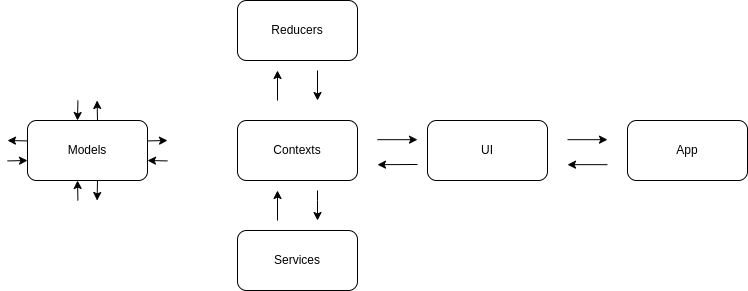
\includegraphics[width=0.5\textwidth]{diagrama_flujo_reducer.png}
    \caption{Diagrama de flujo de la arquitectura con el patrón de diseño de Reducer}
  \end{center}
\end{figure}

\end{document}
